The simulation result will be compared with the result on the paper \cite{krishnapriya2014}. \\
The simulations were performed by varying two parameters:

\begin{itemize}
    \item \texttt{t\_d}: Membrane thickness
    \item \texttt{P\_x}: Applied external pressure
\end{itemize}

\noindent
The quantities of interest to be extracted from the results are:

\begin{itemize}
    \item \textbf{Displacement}: Membrane displacement
    \item \textbf{Stress}: Membrane von Mises stress
    \item \textbf{Sensitivity}: Maximum displacement per unit applied pressure
\end{itemize}

\subsection{Diaphragm Displacement}
The first quantity compared with the results reported in the reference paper is the membrane displacement. \\
The maximum displacement values for both structures differ from those reported in the paper. \\
This difference is expected, since the geometrical details of the holes and corrugations are not fully specified in the paper, leading to differences between the simulated and reference structures. \\
The most relevant observation is that, in the reference paper, the difference in maximum displacement between the two structures is significantly larger than in the simulations. \\
In fact, the maximum displacement reported in \cite{krishnapriya2014} ranges from \(0.7169 \; \mu m\) for the perforated diaphragm structure to \(0.4875 \; \mu m\) for the perforated backplate structure, whereas in the simulations the values range from \(0.585 \; \mu m\) to \(0.551 \; \mu m\), respectively, as shown in \autoref{fig:3d_displacement_module}.

\begin{figure}[h!]
    \centering
    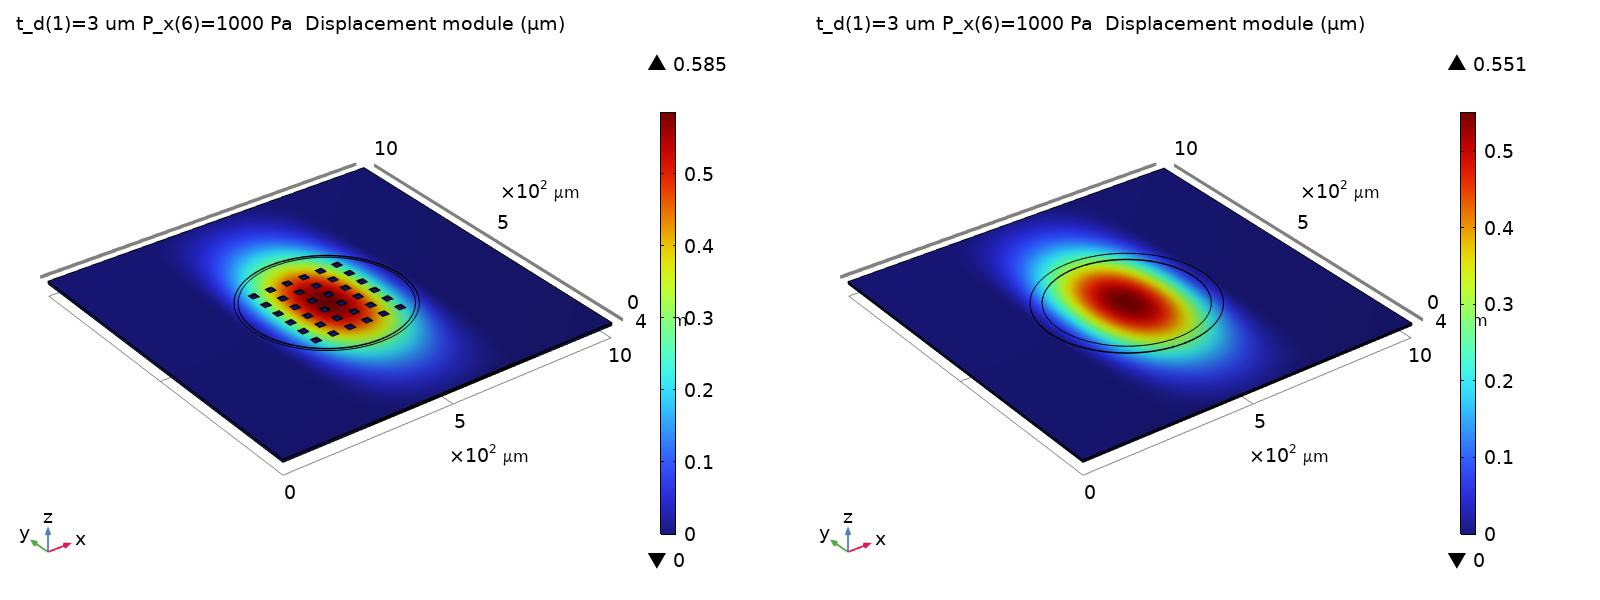
\includegraphics[width=1\linewidth]{img/3d_displacement_module.jpg}
    \caption{Displacement magnitude for both structures: \\
    left is perforated diaphragm structure, right is perforated back structure}
    \label{fig:3d_displacement_module}
\end{figure}

\noindent
It is important to specify that the displacement shown in \autoref{fig:3d_displacement_module} has been obtained with a diaphragm thickness (\texttt{t\_d}) of \(3 \; \mu m\), an air gap (\texttt{h\_air}) of \(1 \; \mu m\), and an applied external pressure (\texttt{P\_x}) of \(1000 \; \text{Pa}\), which are the same values used in the reference paper. \\
The difference in displacement values is due to the presence of holes in the membrane, which mechanically weaken the structure and result in a larger displacement under the same applied load. \\
Although the holes weaken the structure, the deformation trend as a function of position remains similar for both configurations. \\
To verify this, the displacement along a line on the diaphragm surface has also been evaluated.

\begin{figure}[h!]
    \centering
    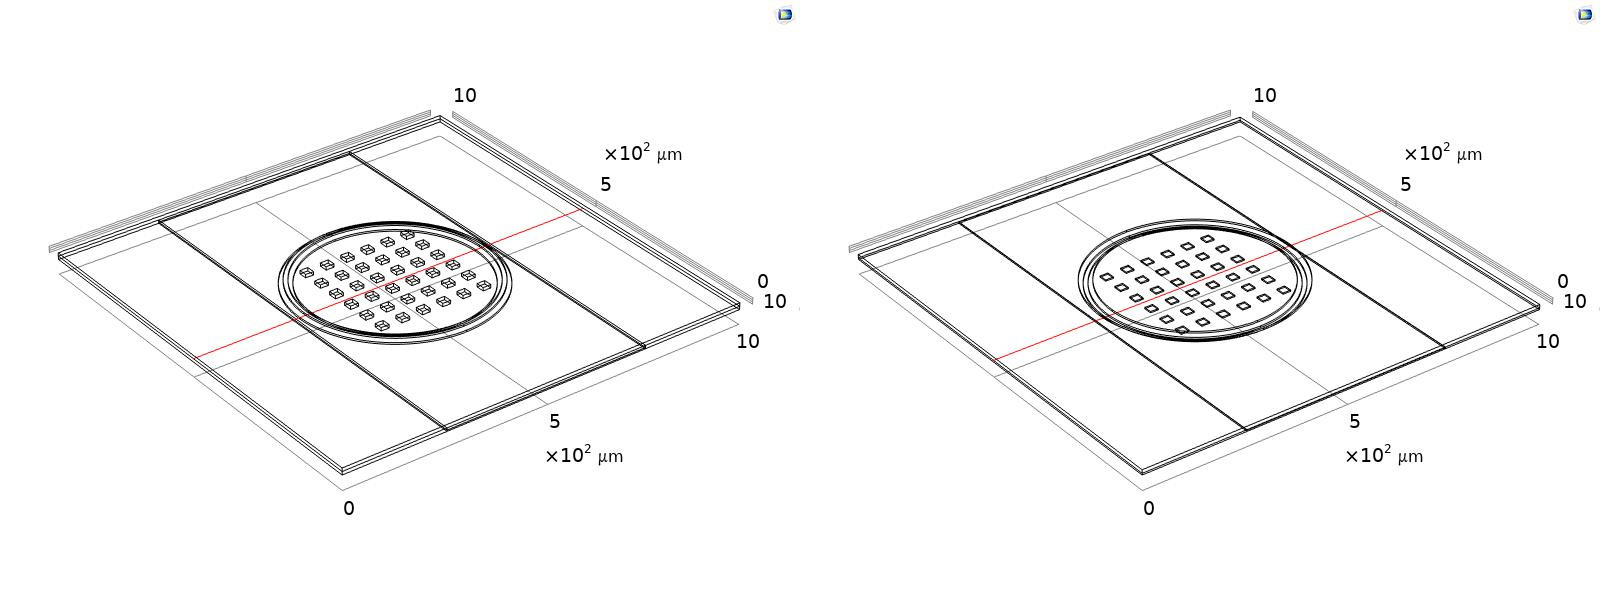
\includegraphics[width=1\linewidth]{img/center_line_visualization.jpg}
    \caption{Line along which the displacement is evaluated: \\
    left is perforated diaphragm structure, right is perforated back structure}
    \label{fig:center_line_visualization}
\end{figure}

\begin{figure}[h!]
    \centering
    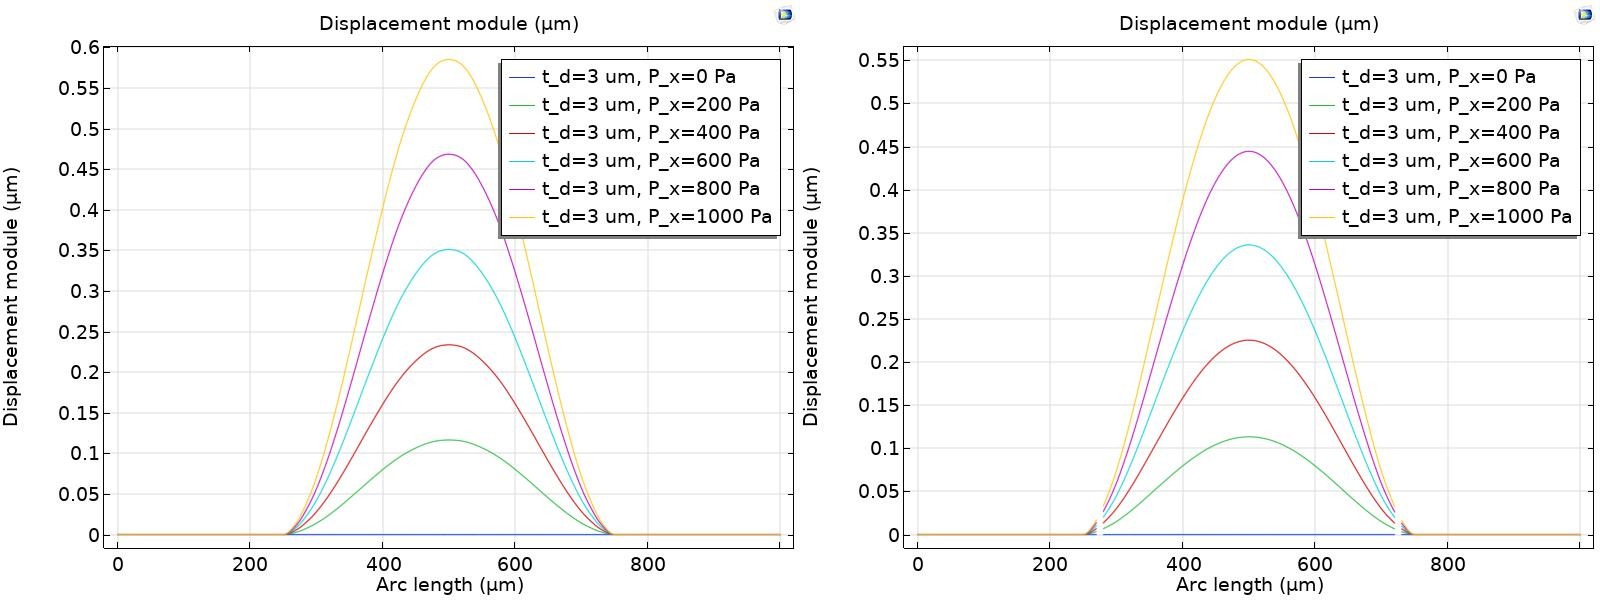
\includegraphics[width=1\linewidth]{img/center_line_displacement.jpg}
    \caption{Center-line displacement as a function of arc length, parameterized by applied pressure: \\
    left is perforated diaphragm structure, right is perforated back structure}
    \label{fig:center_line_displacement}
\end{figure}

\newpage
\noindent
As shown in \autoref{fig:center_line_displacement}, the displacement along the arc length follows the same trend for both structures; however, the perforated diaphragm structure always have a higher maximum displacement, as we expected. \\
It can also be observed that, by reducing the applied pressure, the difference in maximum displacement between the two structures becomes less significant. \\
Can be also interesting to analyze the behavior of the maximum displacement as a function of diaphragm thickness.

\begin{figure}[h!]
    \centering
    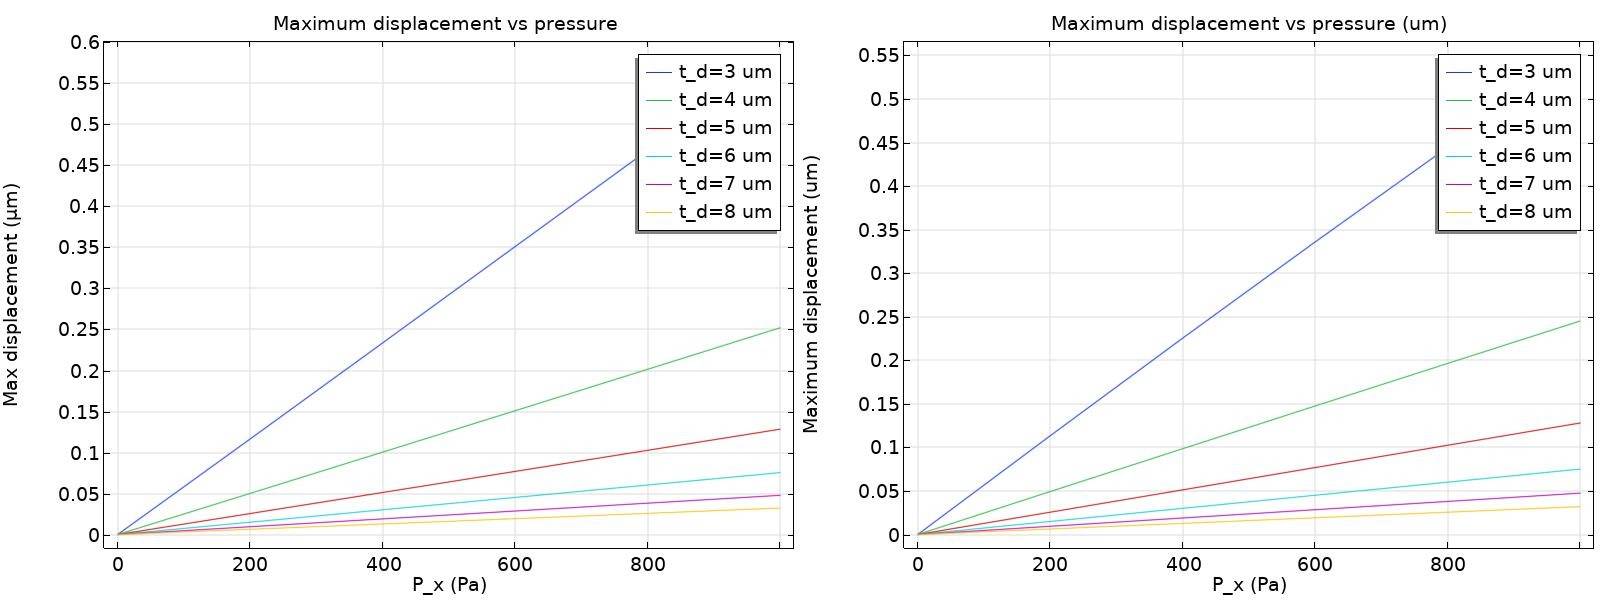
\includegraphics[width=1\linewidth]{img/maximum_disp_vs_pressure.jpg}
    \caption{Maximum center-line displacement as a function of applied pressure, parameterized by diaphragm thickness: \\
    left is perforated diaphragm structure, right is perforated back structure}
    \label{fig:maximum_disp_vs_pressure}
\end{figure}

\noindent
As shown in \autoref{fig:maximum_disp_vs_pressure}, the maximum displacement can be approximated as a linear function of pressure for the range of pressures and diaphragm thicknesses considered. \\
The displacement is always higher for the perforated diaphragm structure (concordant result with \cite{krishnapriya2014}); however, increasing the diaphragm thickness reduces the slope of the function, resulting in a smaller difference in displacement between the two structures. \\
Due to the linear trend of the function, reducing the applied pressure also leads to a decrease in displacement and, consequently, to a smaller difference in displacement between the two structures; this effect can also be observed in \autoref{fig:center_line_displacement}.

\subsection[Electromechanical Effects of Applied Bias Voltage]{Electromechanical Effects of \\ Applied Bias Voltage}

The voltage applied to the structure to measure the capacitance of the sensor generates an electric field in the air gap of the microphone, which attracts the membrane toward the bottom plate, causing a mechanical displacement of the diaphragm. \\
An interesting analysis consists in evaluating the membrane displacement induced only by the applied voltage (\autoref{fig:3D_voltage_displacement} and \autoref{fig:center_line_voltage_displacement}). \\
The simulation was performed without external pressure, with a diaphragm thickness (\texttt{t\_d}) of \(3 \; \mu m\), and with an applied voltage (\texttt{V\_x}) of \(1 \; V\). \\
As shown in \autoref{fig:3D_voltage_displacement}, the maximum displacement is \(7.68 \cdot 10^{-4} \; \mu m\) for the perforated diaphragm structure and \(1.09 \cdot 10^{-3} \; \mu m\) for the perforated backplate structure.

\begin{figure}[h!]
    \centering
    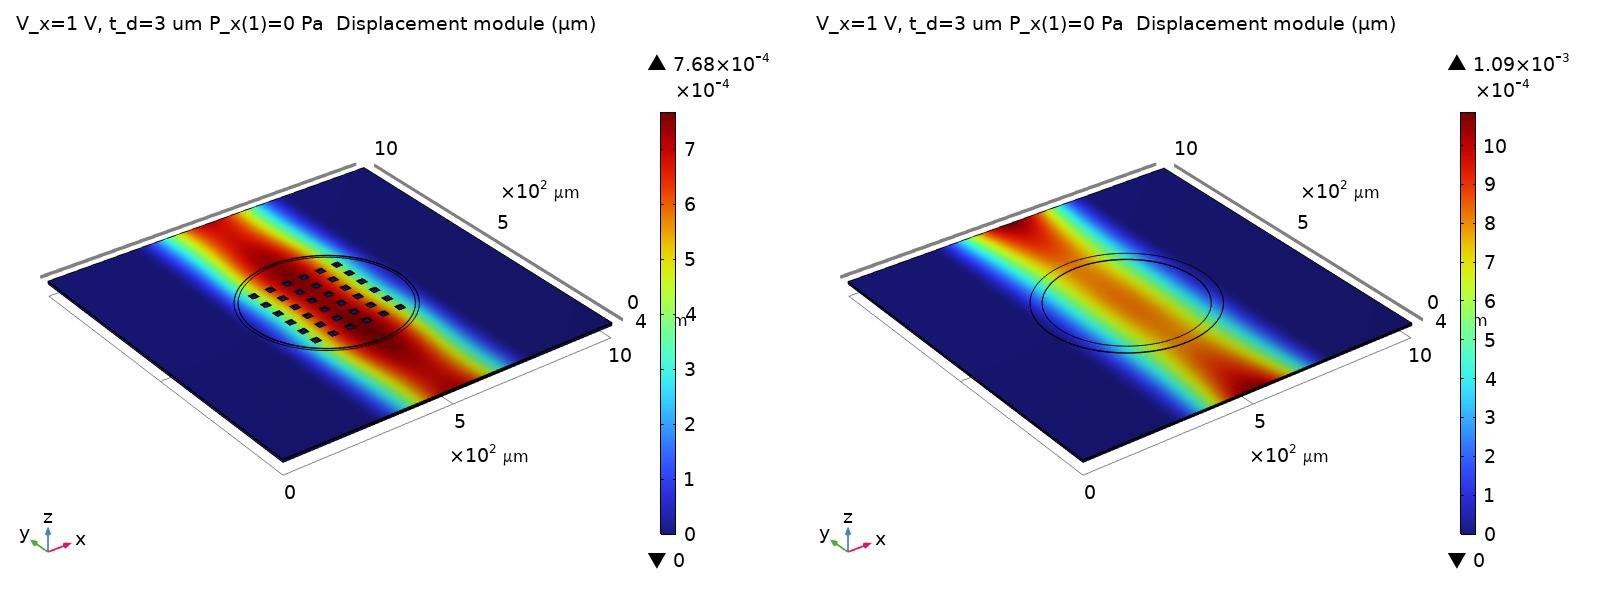
\includegraphics[width=1\linewidth]{img/3D_voltage_displacement.jpg}
    \caption{Displacement magnitude obtained without external pressure, induced only by the applied voltage: \\
    left is perforated diaphragm structure, right is perforated back structure}
    \label{fig:3D_voltage_displacement}
\end{figure}

\begin{figure}[h!]
    \centering
    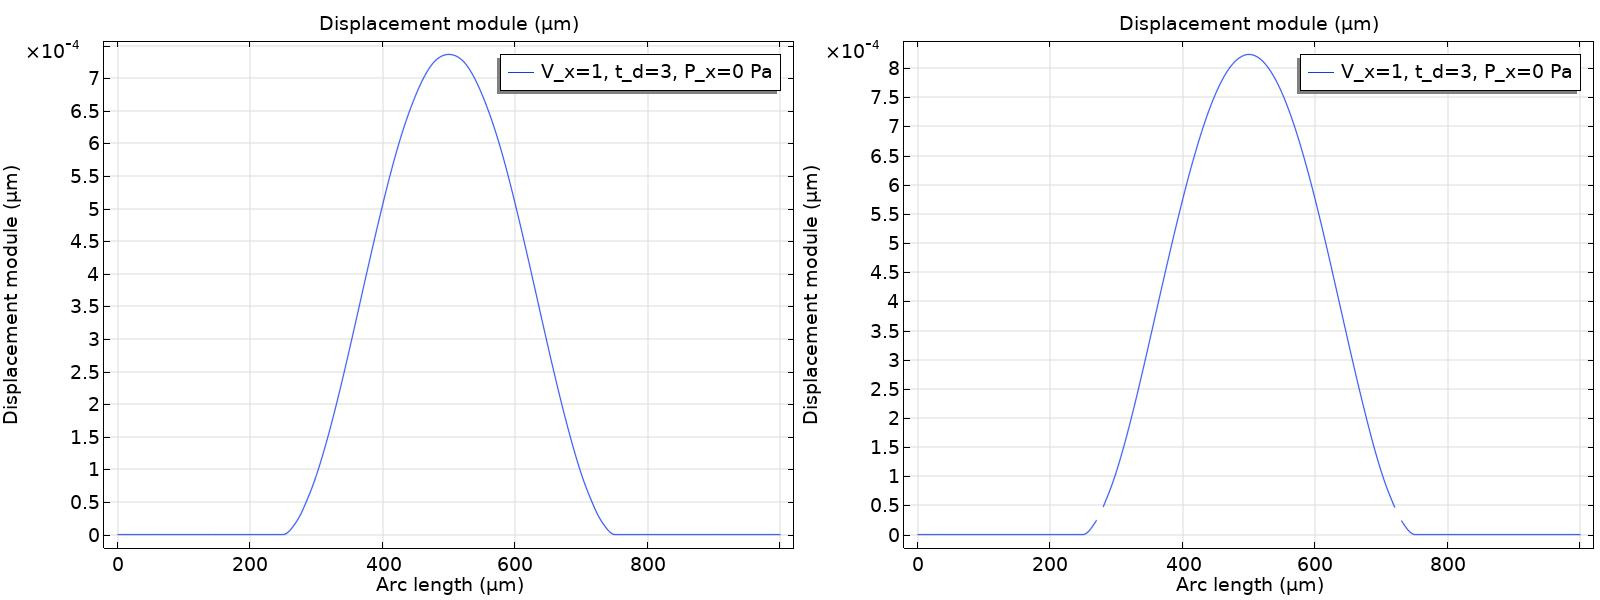
\includegraphics[width=1\linewidth]{img/center_line_voltage_displacement.jpg}
    \caption{Center-line displacement obtained without external pressure, induced only by the applied voltage: \\
    left is perforated diaphragm structure, right is perforated back structure}
    \label{fig:center_line_voltage_displacement}
\end{figure}

\noindent
These values do not match those shown in \autoref{fig:center_line_voltage_displacement} because the maximum displacement reported in \autoref{fig:3D_voltage_displacement} considers the entire membrane domain. In particular, the displacement at the membrane edges is greater than at its center. \\
For pressures greater than \(100 \; Pa\), the displacement values for both structures are more than two orders of magnitude larger; therefore, the displacement generated by the applied voltage is negligible in comparison. \\
Now, with bias voltage selected of \(1 \; V\) let's check the variation of Maxwell capacitance with pressure for both structures (\autoref{fig:Capacitance_vs_pressure})

\begin{figure}[h!]
    \centering
    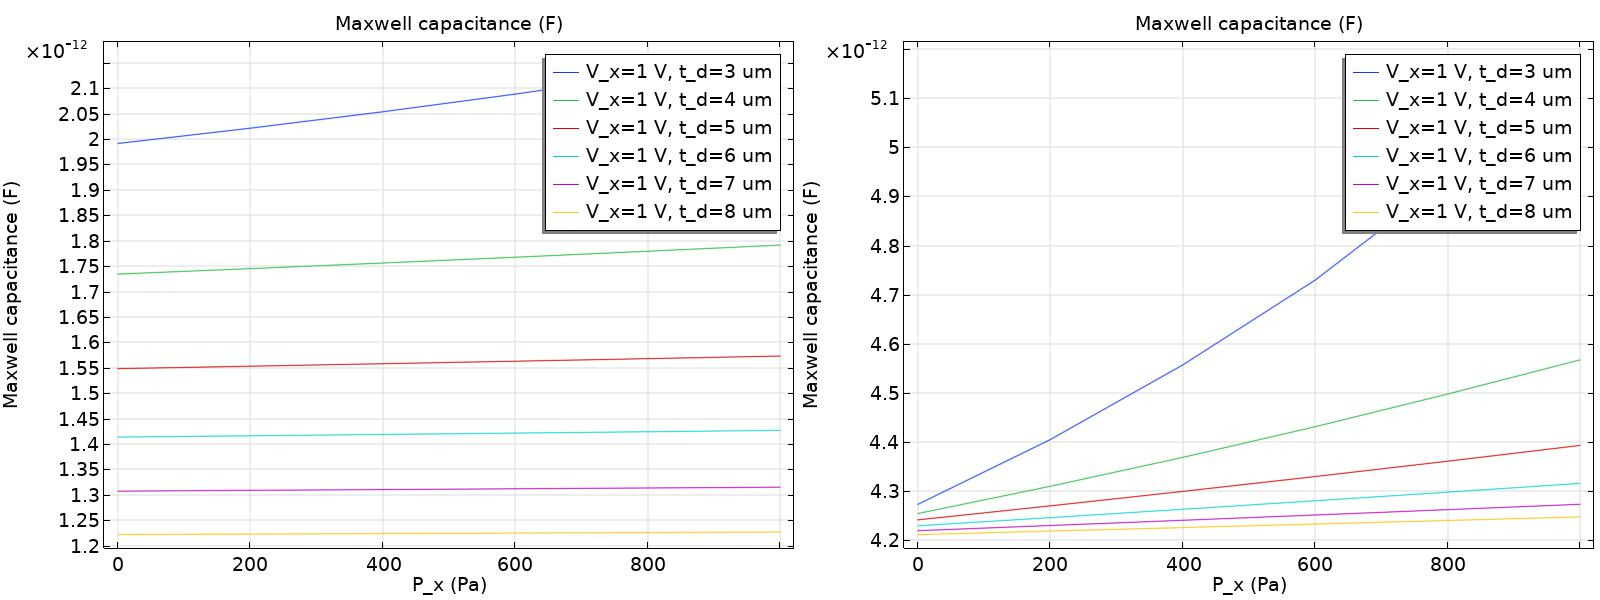
\includegraphics[width=1\linewidth]{img/Capacitance_vs_pressure.jpg}
    \caption{Capacitance vs external pressure applied: \\
    left is perforated diaphragm structure, right is perforated back structure}
    \label{fig:Capacitance_vs_pressure}
\end{figure}

\noindent
As shown in \autoref{fig:Capacitance_vs_pressure}, the capacitance is slightly higher for the perforated back structure, although the difference is not significant. \\
The most relevant aspect is the noticeable difference in capacitance sensitivity between the two configurations.

\begin{equation}
    \begin{aligned}
        \left. S_P^C \right|_{\text{perf. diap.}} & = \left. \frac{\partial C}{ \partial P} \right|_{\text{perf. diap.}} \\ 
        \frac{2.1663-1.991}{1000} \; \frac{pF}{Pa} & \simeq 0.1753 \cdot 10^{-3} \;\frac{pF}{Pa}
    \end{aligned}
    \label{eq:S_perf_diap}
\end{equation}

\begin{equation}
    \begin{aligned}
        \left. S_P^C \right|_{\text{perf. back}} & = \left. \frac{\partial C}{ \partial P} \right|_{\text{perf. back}} \\ 
        \frac{5.1897-4.2719}{1000} \; \frac{pF}{Pa} & \simeq 0.9178 \cdot 10^{-3} \; \frac{pF}{Pa}
    \end{aligned}
    \label{eq:S_perf_back}
\end{equation}

\noindent
The values in \cref{eq:S_perf_back} and \cref{eq:S_perf_diap} has been evaluated assuming a diaphragm thickness (\texttt{t\_d}) of \(3 \; \mu m\), a bias voltage (\texttt{V\_x}) of \(1 \; V\) and a linear approximation of the capacitance–pressure relationship.

\subsection{Diaphragm von Mises Stress}

The other quantity compared with the results reported
in the reference paper is the membrane stress.

\begin{figure}[h!]
    \centering
    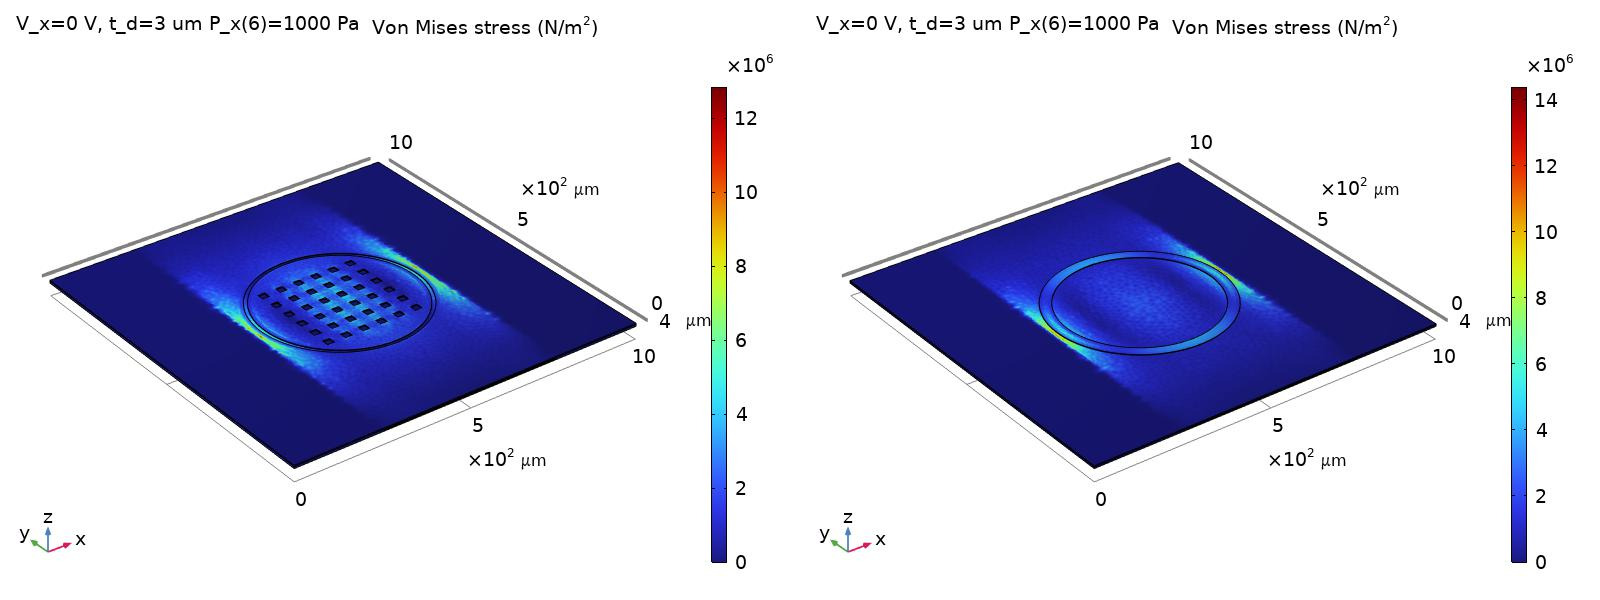
\includegraphics[width=1\linewidth]{img/3d_stress.jpg}
    \caption{von Mises stress for both structures: \\
    left is perforated diaphragm structure, right is perforated back structure}
    \label{fig:3d_stress}
\end{figure}

\noindent
As shown in \autoref{fig:3d_stress}, the maximum stress is located between the lateral edges and the corrugation of the membrane. \\
Within the corrugation, the stress is primarily concentrated at the center, while in the perforated diaphragm structure it increases near the edges of the holes. \\
The computed maximum stress is not fully representative, since the quantity of interest is the stress within the corrugation of the membrane. \\
However, the result is influenced by a stress peak at the membrane edge. \\
To better evaluate both the peak value and the stress distribution within the membrane, the stress profile along the center line has been analyzed. \\
The line along the stress has been evaluated is the same used for the displacement, shown in \autoref{fig:center_line_visualization}.

\begin{figure}[h!]
    \centering
    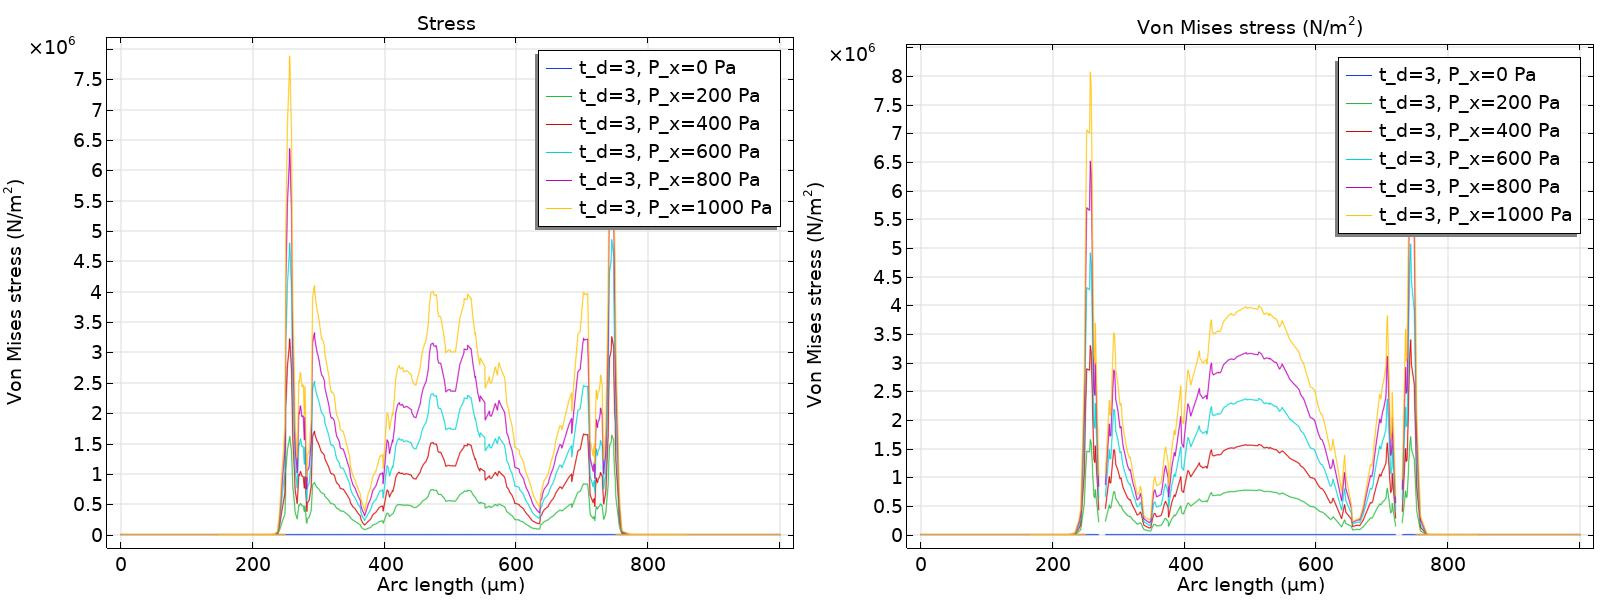
\includegraphics[width=1\linewidth]{img/center_line_von_mises_stress.jpg}
    \caption{Center-line von Mises stress as a function of arc length, parameterized by applied pressure: \\
    left is perforated diaphragm structure, right is perforated back structure}
    \label{fig:center_line_von_mises_stress}
\end{figure}

\newpage
\noindent
As we can see in \autoref{fig:center_line_von_mises_stress}, for the perforated diaphragm structure, the stress increases near the edges of the holes and decreases with increasing distance from them. \\
In contrast, for the perforated back structure, the stress distribution follows a trend that is closer to a quadratic profile. \\
Within the membrane region delimited by the corrugation, the maximum stress is nearly the same for both structures; the only difference lies in the stress distribution along the center line. \\
The stress also varies along the z-axis within the membrane (see \autoref{fig:MEMS_microphone_structure} for the axis orientation). The values shown in \autoref{fig:center_line_von_mises_stress} are evaluated along a line at the top surface of the membrane. \\
To obtain a more accurate estimate, excluding the stress peak near the lateral edges, the maximum stress at the top surface has been evaluated within the region delimited by the corrugation, that is also the area where the external pressure is applied (see \autoref{fig:applyed_pressure}).

\begin{figure}[h!]
    \centering
    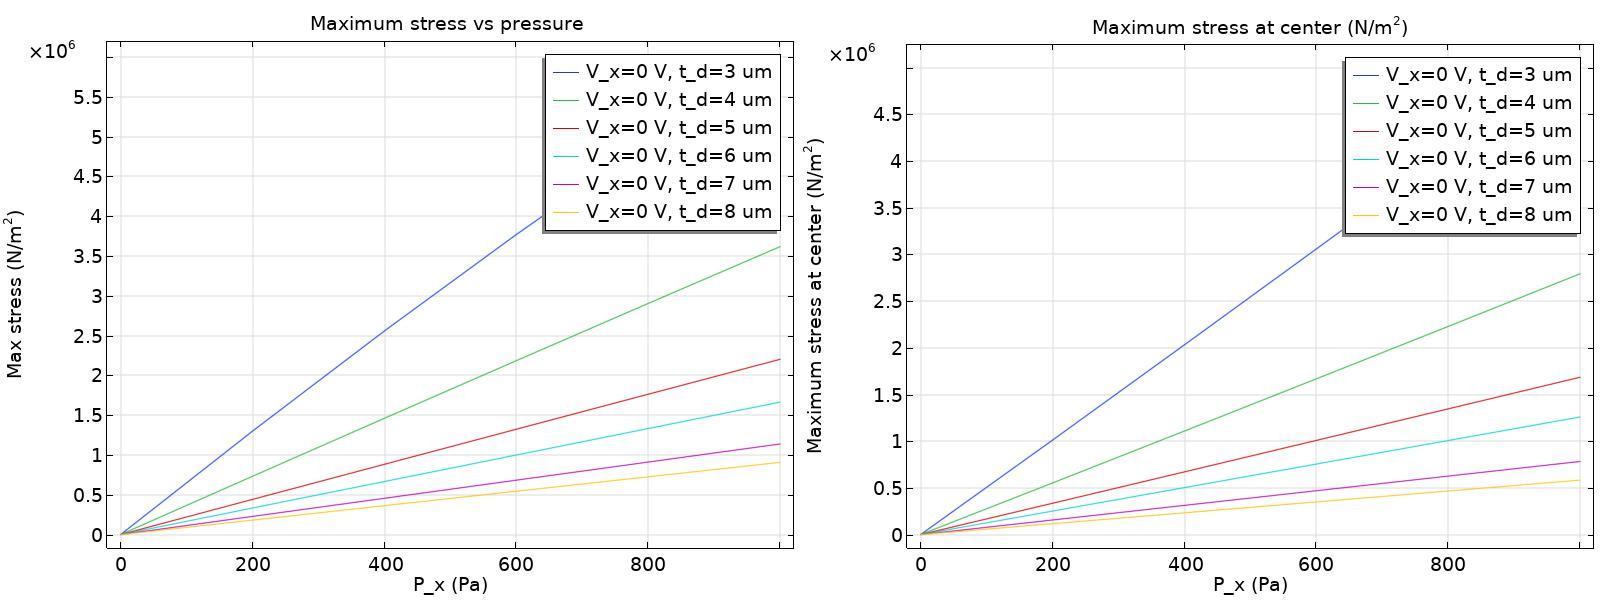
\includegraphics[width=1\linewidth]{img/maximum_stress_center_line.jpg}
    \caption{Maximum von Mises stress as a function of pressure applied, parametrized by diaphragm thickness: \\
    left is perforated diaphragm structure, right is perforated back structure}
    \label{fig:maximum_stress_center_line}
\end{figure}

\noindent
The stress, although less regular function than the displacement (along the center line), has a maximum value within the membrane that shows an approximately linear dependence on the applied pressure.

\newpage
\subsection[Displacement Sensitivity]{Diaphragm Displacement \\ Sensitivity}

The last parameter to be calculated is the displacement sensitivity of the membrane defined as \cref{eq:disp_sensitivity_definition}

\begin{equation}
    S_P^y = \frac{\text{maximum displacement}}{\text{pressure applied}} = \frac{max(|y|)}{P}
    \label{eq:disp_sensitivity_definition}
\end{equation}

\noindent
The perforated diaphragm structure has a weaker membrane; therefore, under the same applied pressure, it respond with a larger displacement. \\
For this reason, its displacement sensitivity is higher than that of the perforated back structure. \\
To verify this has been computed the displacement sensitivity as function of the applied pressure. \\
The maximum displacement value has been evaluated on the entire membrane domain for both structures (same method used to compute the maximum displacement on \autoref{fig:maximum_disp_vs_pressure})

\begin{figure}[h!]
    \centering
    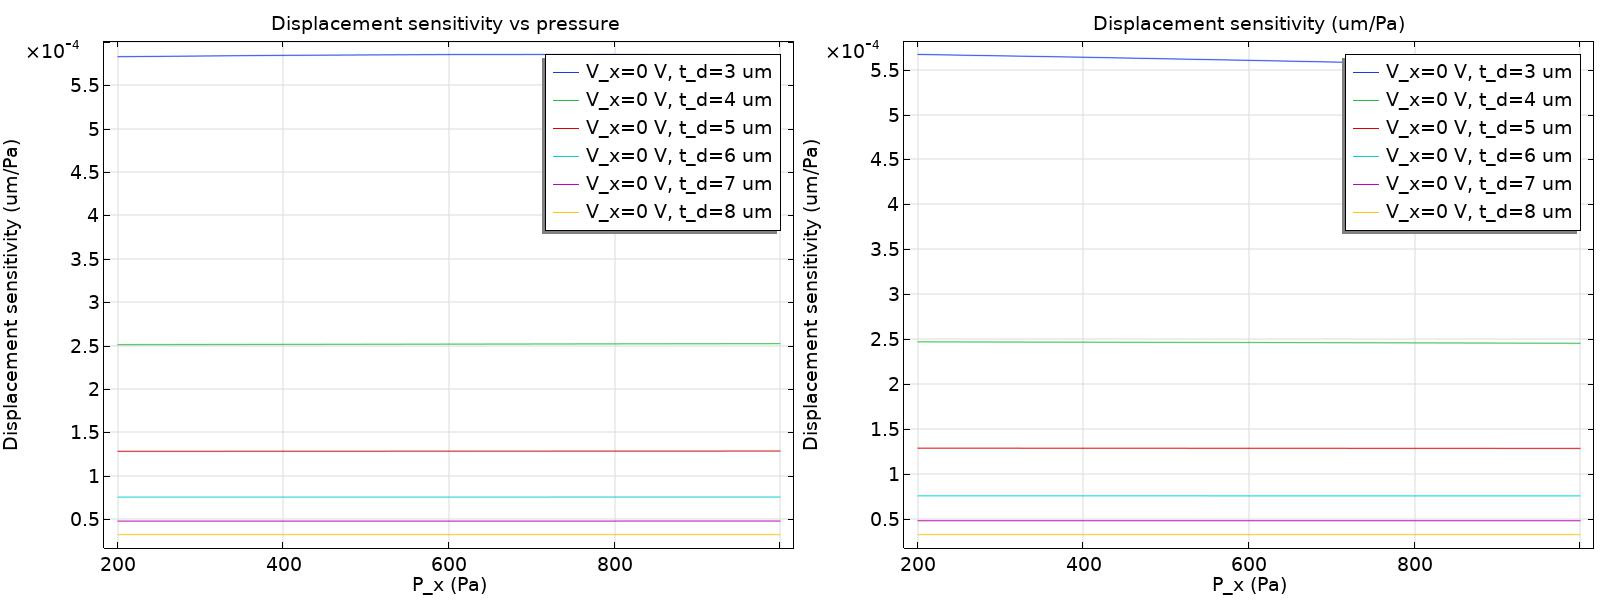
\includegraphics[width=1\linewidth]{img/displacement_sensitivity_parametrized.jpg}
    \caption{Maximum diaphragm displacement sensitivity as a function of pressure applied, parametrized by diaphragm thickness: \\
    left is perforated diaphragm structure, right is perforated back structure}
    \label{fig:displacement_sensitivity_parametrized}
\end{figure}

\noindent
As expected (\autoref{fig:displacement_sensitivity_parametrized}), the displacement sensitivity of the perforated diaphragm structure is higher than that of the perforated back structure. \\
However, due to the small difference in maximum displacement between the two configurations, the sensitivities are comparable. \\
The displacement sensitivity remains nearly constant with respect to pressure. \\
However, to better analyze its trend, the sensitivity was also evaluated with a single diaphragm thickness value.

\begin{figure}[h!]
    \centering
    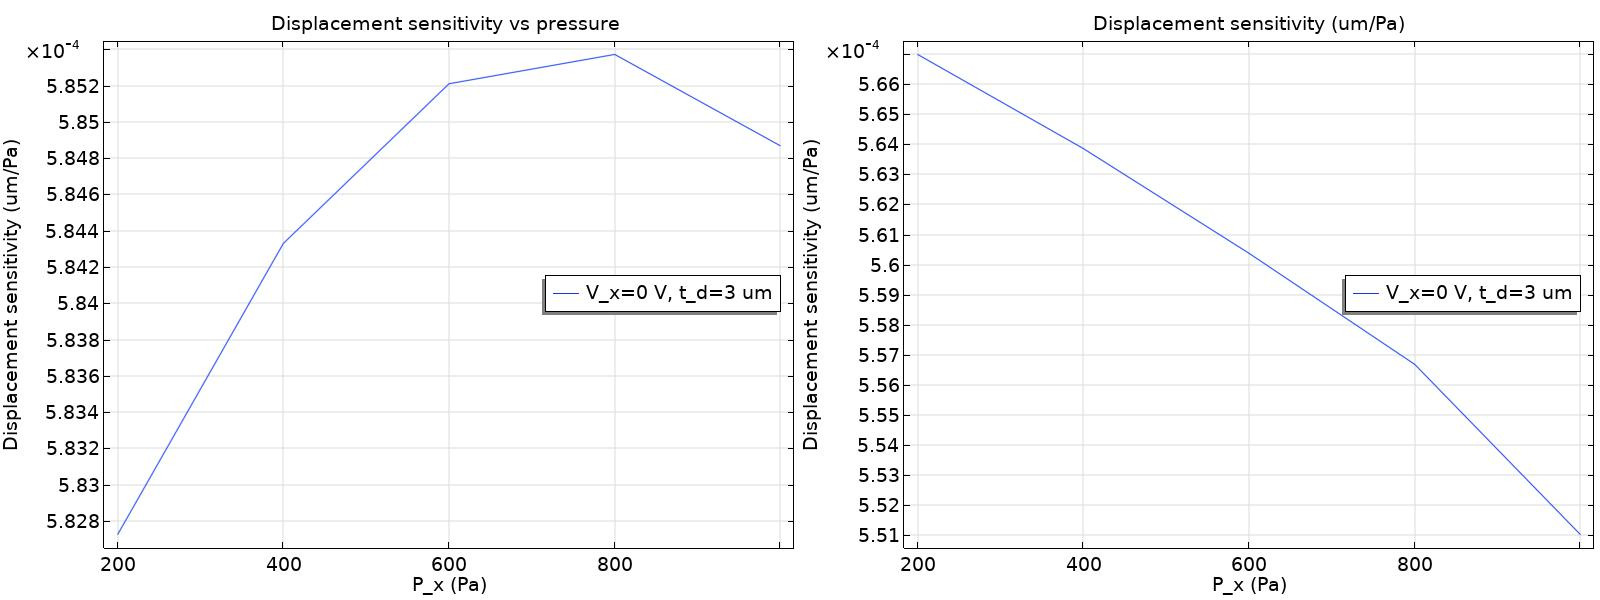
\includegraphics[width=1\linewidth]{img/displacement_sensitivit_trend_t_d=3um.jpg}
    \caption{Maximum diaphragm displacement sensitivity as a function of pressure applied, with a diaphragm thickness (\texttt{t\_d}) of \(3 \; \mu m\): \\
    left is perforated diaphragm structure, right is perforated back structure}
    \label{fig:displacement_sensitivit_trend_t_d=3um}
\end{figure}

\newpage
\noindent
From \autoref{fig:displacement_sensitivit_trend_t_d=3um}, graph obtained with a diaphragm thickness (\texttt{t\_d}) of \(3 \; \mu m\), we can see that for the perforated diaphragm structure the displacement sensitivity has an initially growing trend, which reaches a local maximum and then begins to decrease, and for the perforated back structure the trend is only decreasing. \\
To make a comparison, in the paper \cite{krishnapriya2014} the sensitivity is approximately constant with respect to the applied pressure, similarly to the simulation results. The reported values are \cref{eq:paper_sensitivity_value}

\begin{equation}
    \begin{aligned}
        \left. S_P^y \right|_{\text{perf. diap.}} &\simeq 7 \cdot 10^{-4} \; \mu\text{m}/\text{Pa} \\
        \left. S_P^y \right|_{\text{perf. back}} &\simeq 5 \cdot 10^{-4} \; \mu\text{m}/\text{Pa}
    \end{aligned}
    \label{eq:paper_sensitivity_value}
\end{equation}

The simulation results instead are \cref{eq:computed_sensitivity_value}

\begin{equation}
    \begin{aligned}
        \left. S_P^y \right|_{\text{perf. diap.}} &\in \left[5.82 ,\, 5.86\right]  \; \cdot 10^{-4} \mu\text{m}/\text{Pa} \\
        \left. S_P^y \right|_{\text{perf. back}} &\in \left[5.51 ,\, 5.67\right] \cdot 10^{-4} \; \mu\text{m}/\text{Pa}
    \end{aligned}
    \label{eq:computed_sensitivity_value}
\end{equation}

\noindent
As expected, the sensitivity values obtained from the simulations are of the same order of magnitude and show good agreement with the literature results for both structures.
This is because, as shown in \autoref{fig:3d_displacement_module}, the maximum displacement is almost the same in both cases; for this reason also the sensitivity values are similar. \\ 
The perforated back structure gives a maximum displacement that is close to the value reported in \cite{krishnapriya2014}. In contrast, the perforated diaphragm structure shows a larger difference. \\
For this reason, the results of the perforated back structure are closer to the reference paper values, while the other configuration differs more from them.

\newpage
